\newpage
\section{Introduction}
\subsection{Network Technology: from local to global}
\subsubsection{Network Hardware}
依据传输技术(transmission technology)与规模(scale)分类. 

传输技术分两种: 
\begin{itemize}
    \item Broadcast links (Multicasting多播)
    \subitem 链路被所有机器共享 (有线+无线, 长距离只能用有线)
    \subitem 无线网络是典型的 broadcast links
    \subitem 地址全部是1表示将数据包寻址到所有目的地地址字段(向所有人发信息), 地址全是0表示初始/未分配地址. 
    \item Point-to-point links
    \subitem 有很多路径, 选择基于路由算法. %TODO 明确定义
\end{itemize}

依据规模分类: 距离是重要指标. 
\begin{figure}[!htb]
    \centering
    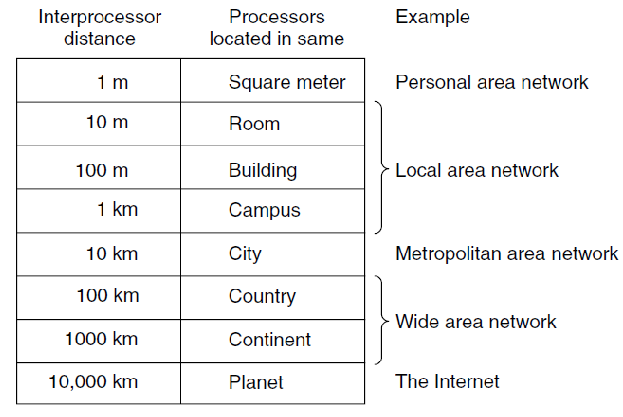
\includegraphics[width=0.309\textwidth]{pic/CN1/scale}
    \caption{scale}
\end{figure}

\paragraph{Communication Links} e.g.
\begin{itemize}\small
    \item Coaxial cable (telephone)
    \item Copper wire (TV)
    \item Fiber optics (the backbone the PSTN, Public Switched Telephone Network)
    \item Radio spectrum (cellphone)
\end{itemize}

Different links can transmit data at different rates, with \textbf{the transmission rate} of a link measured in bits/second. 传输速率以 bits/second 衡量. 每个 bits 的持续时间 (duration, seconds/bit) 就是传输速率的倒数. 

高的传输速率易被噪声影响, 比如 持续 10ms 的噪声, 影响 100bits/s 的 2bits, 1kbits/s 的 11btis. 

\paragraph{Personal Area Network(PAN)} e.g. Bluetooth networks use the master-slave paradigm. 

\paragraph{Loacl Area Network(LAN)} 是 broadcast link, 有问题, 处理分两种:
\begin{itemize}
    \item Static: time slot (TDM) and FDM, 时分 or 频分. 
    \item Dynamic allocation methods for a common channel are either centralized and decentralized. 动态分配, 要么中心化, 要么去中心化. 
\end{itemize}

\paragraph{Home Networks} 以后可能会有, 家庭网络. 
\paragraph{Metropolitan Area Network(MAN)} e.g. 
\begin{itemize}
    \item Wired: cable television
    \item Wireless: IEEE 802.16 (WiMax), telephone network
\end{itemize}

有两种方式: 
\begin{itemize}
    \item VPN (Virtual Private Network) 自建
    \subitem 优点: reuse of resource 资源重利用
    \subitem 缺点: 调用底层资源时受限
    \item ISP (Internet Service Provider) 租用资源
\end{itemize}


\subsection{Examples of Networks}
\subsubsection{The Internet}
鼻祖: The ARPANET, 后面 NSFNET, 然后 Internet. 

层级结构网络不安全, 鲁棒性低. 分布式网络更安全. 

\paragraph{ARPANET} 诞生于 1969, 分两块 subnet 与 host. 
\begin{figure}[!htb]
    \centering
    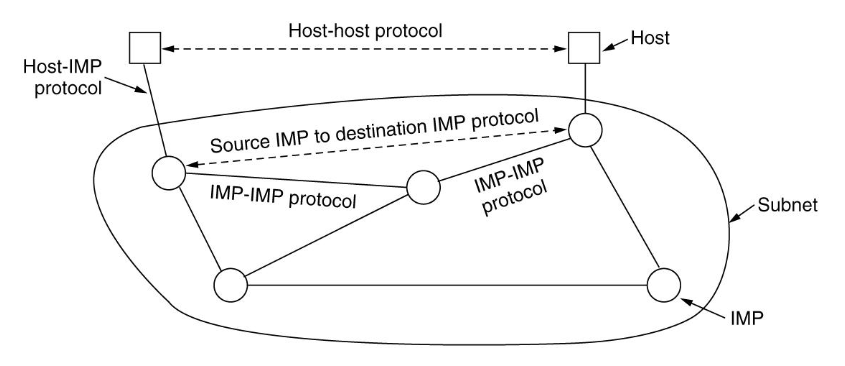
\includegraphics[width=0.309\textwidth]{pic/CN1/ARPANET.png}
    \caption{ARPANET}
\end{figure}

\paragraph{NSFNET} The path a packet takes through the internet depends on the peering choices of the ISPs. 

\begin{enumerate}
    \item 最大的ISP: Tier 1 ISP
    \item 下级的 ISP
    \item 家庭之类的, DSL (Digital Subscriber Line) 宽带?
\end{enumerate}

\paragraph{The Internet’s Architecture}从层级到扁平 %TODO 补图 P51-52

\begin{figure}[!htb]
    \centering
    \includegraphics[width=0.42\textwidth]{pic/CN1/the Internet’s Architecture}
    \caption{the Internet’s Architecture}
\end{figure}

\subsubsection{Mobile networks}
\begin{figure}[!htb]
    \centering
    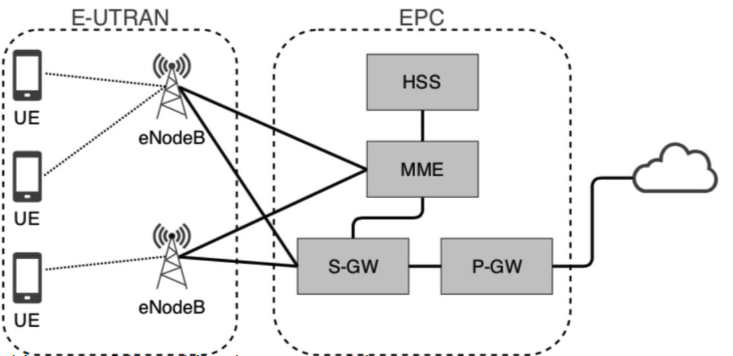
\includegraphics[width=0.42\textwidth]{pic/CN1/Mobile Networks}
    \caption{Mobile Networks}
\end{figure}

\begin{itemize}\small
    \item E-UTRAN (Evolved UMTS Terrestrial Radio Access Network)
    \item EPC (Evolved Packet Core)
    \subitem HSS (Home Subscriber Server)
    \subitem P-GW (Packet Data Network Gateway): 直连 internet
    \subitem S-GW (Serving Network Gateway)
\end{itemize}

\paragraph{Frequency reuse} (频率重用)无线电是稀缺资源, 需要政府 license 进行使用. 把通信区域分块, 设计为蜂窝网络. 理论依据: Cellular Concept %TODO 补图 %TODO 整理下这个

\begin{figure}[!htb]
    \centering
    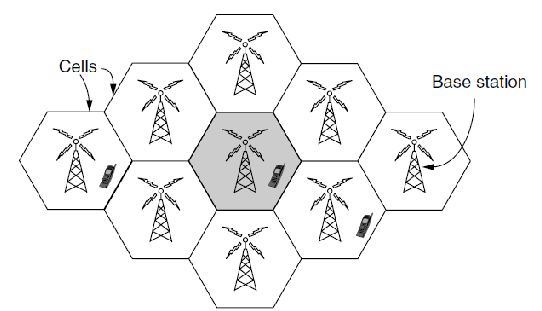
\includegraphics[width=0.309\textwidth]{pic/CN1/frequency reuse}
    \caption{Frequency reuse}
\end{figure}

但 3G 可以每一个cell用所有频率. 

\paragraph{Handover} 不同基站的转移. 

\paragraph{SIM} (Subscriber Identity Module) a removable chip

\paragraph{Evolution of Mobile Networks} 主要区别: 依据频谱分类. 
\begin{enumerate}
    \item First-Generation (1G) 
    \item Second-Generation (2G)
    \item Third-Generation (3G)
    \item 4G
    \item 5G
\end{enumerate}

\paragraph{Packet Switching vs. Circuit Switching} \quad
\begin{itemize}
    \item Packet switching: 数据包来选择路径
    \item Circuit switching: 建立路径传输数据
\end{itemize}

\subsubsection{Wireless networks (802.11 WiFi)}
为LAN制定的标准, 限制传输功率 (transmit power) 以允许不同的设备共存. 

\paragraph{APs (Access Points)} 链接有线网, 通信通过 APs 进行. 

\paragraph{Multipath fading} 传输的多个回波可能沿着不同的路径到达接收器. 回波可以相互抵消或增强, 导致接收信号大幅波动.

解决方法: path diversity, 使用多条独立路径传输信息, e.g. 
\begin{itemize}
    \item 在允许的频带内使用不同的频率
    \item 使用不同天线, 可以从不同的方向接受信号(MIMO)
    \item 在不同的时间段重复信息
\end{itemize}

\paragraph{ALOHA} CSMA (Carrier Sense Multiple Access) 为解决同时发送多个传输时的冲突(collision)问题, 也叫 ALOHA. 等待一个随机的时间段后发送. 

\subsection{Network Protocols}
设计目标:
\begin{itemize}
    \item Reliability 可靠性
    \item Resource allocation 资源分配
    \item Evolvability 可进化
    \item Security 安全
\end{itemize}

重要思想: layering (分层)

Connection-oriented vs. connectionless service

Specific service primitives (特殊服务功能)

\subsubsection{Design Goals}
\paragraph{Reliability} 可靠, 有 Error detection 与 Error correction 机制. 可在各中状况下自动寻路.
\paragraph{Resource allocation} 统计多路复用 (Statistical multiplexing). 在网络中每一层出现, 使用 flow control. 使用 congestion control. 
\paragraph{Evolvability} 解耦, 函数端口一直, 具体实现不同. 使用地址或命名进行区别. 不同技术各有优缺. Called internetworking. 
\paragraph{Security} 安全问题与解决. 

\subsubsection{Protocol Layering} 
每一层仅为上一层服务. 在第1层之下是实际通信发生的物理介质. Interface 位于每对相邻层之间. 

\paragraph{Protocol stack} a list of the protocols used by a certain system, one protocol per layer. (某个系统使用的协议列表,每层一个协议. )
\paragraph{Protocol}A protocol defines the format and the order of messages exchanged between two or more communication entities, as well as the actions taken on the transmission and/or receipt of a message or other event. (协议定义了两个或多个通信实体之间交换的消息的格式和顺序, 以及在发送和/或接收消息或其他事件时采取的行动. )

\begin{figure}[!htb]
    \centering
    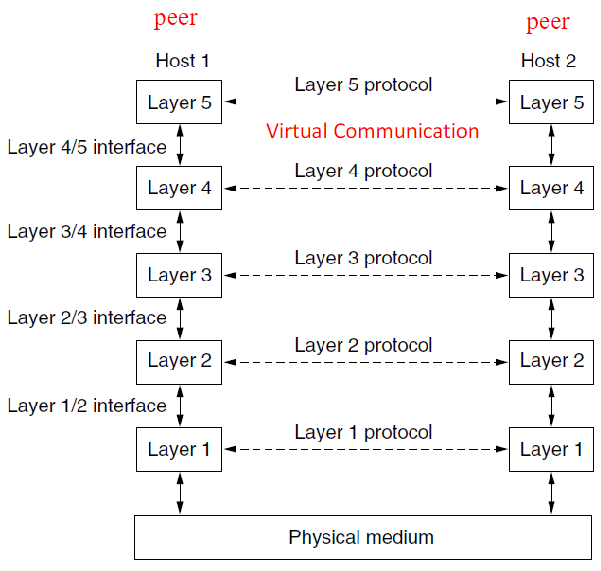
\includegraphics[width=0.309\textwidth]{pic/CN1/Layers}
    \caption{Layers, protocols and interfaces}
\end{figure}

\begin{figure}[!htb]
    \centering
    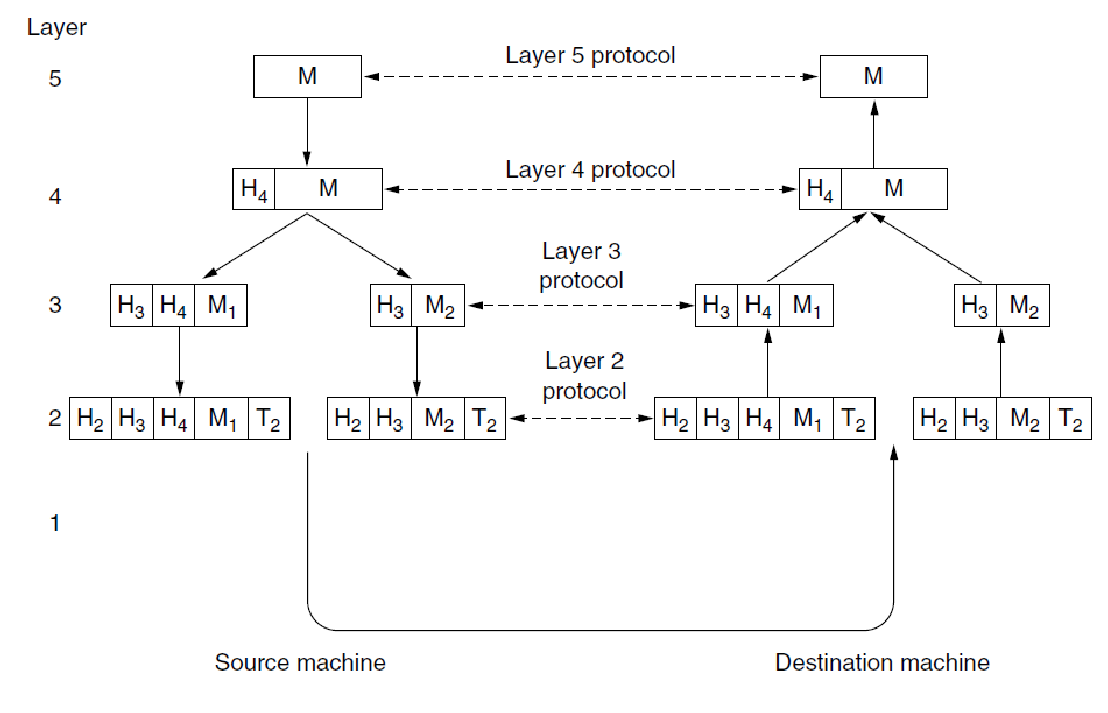
\includegraphics[width=0.42\textwidth]{pic/CN1/information flow}
    \caption{Example information flow}
\end{figure}

\paragraph{Connection-Oriented vs. Connectionless Service}\quad

\begin{itemize}
    \item Connection-oriented service: 建立链接, 使用链接, 释放链接. 
    \item Connectionless service
    \begin{itemize}
        \item 直发 Cut-through switching
        \item 存储后转发 Store-and-forward switching
    \end{itemize}
\end{itemize}

\paragraph{Service Primitives}等实验讲, 服务的函数. 

\paragraph{Services vs. Protocols}Services 是层与层, Protocols 是 host 与 host. 可以随意更改 Protocols, 但是不能更改用户可见的Services. 

\begin{figure}[!htb]
    \centering
    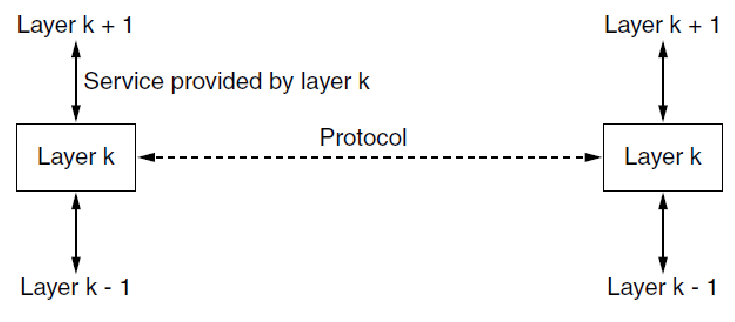
\includegraphics[width=0.42\textwidth]{pic/CN1/Services vs. Protocols}
    \caption{Services vs. Protocols}
\end{figure}

\subsection{Reference Models}
\subsubsection{The OSI reference model}
OSI 是参考模型, 有七层:
\begin{enumerate}
    \item The physical layer
    \item The data link layer
    \item The network layer
    \item The transport layer
    \item The session layer
    \item The presentation layer
    \item The application layer
\end{enumerate}
OSI 并不是真正网络结构, 只是参考, 没有根基. 

\begin{figure}[!htb]
    \centering
    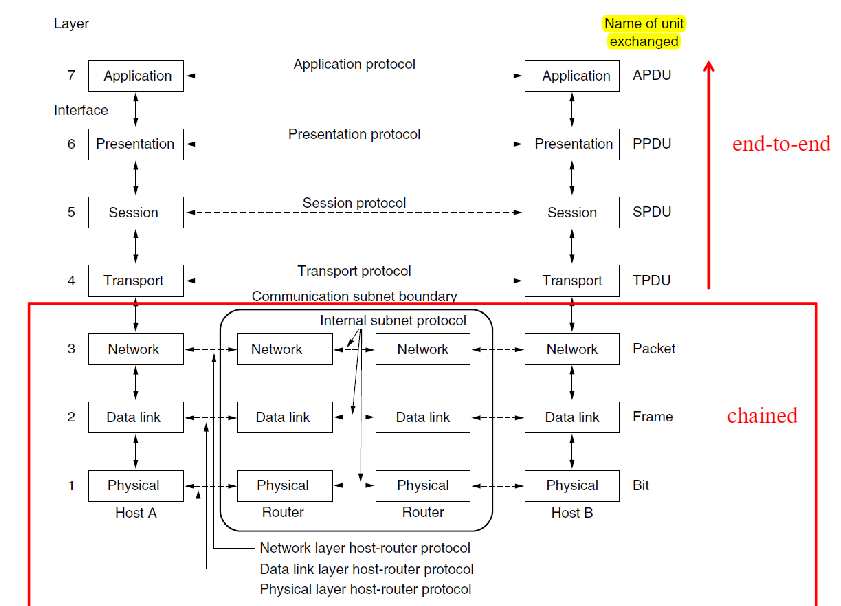
\includegraphics[width=0.42\textwidth]{pic/CN1/OSI.png}
    \caption{The OSI reference model}
\end{figure}

最小传输单元:
\begin{itemize}
    \item The physical layer 是 bit
    \item The data link layer 的是 frame
    \item The network layer 是 packet
\end{itemize}

1-3 层是链路(chained), 可以被打开? %TODO 链路的概念

\paragraph{Physical Layer}: 最底层. 

传输媒介: guided media or unguided media (有型与无型). 

数字调制和多路复用: TDM, FDM, CDM

\paragraph{Data Link Layer}三个功能:
\begin{enumerate}
    \item Framing 分帧
    \item Flow Control
    \item Error Control
\end{enumerate}
涉及如何控制对共享频道的访问. 

\paragraph{Network Layer}: 转发包. 涉及:
\begin{itemize}
    \item 路由算法
    \item 网络协议: IPv4, IPv6
    \item Congestion control algorithms 与 Quality of services 自己看 %TODO
\end{itemize}

\paragraph{Transportation Layer}: 端到端
\begin{itemize}
    \item Connectionless Transport Protocol: UDP
    \item Connection-Oriented Transport Protocol: TCP
\end{itemize}

\paragraph{Session Layer and Presentation Layer}可放弃.jpg

\paragraph{Application Layer}协议:
\begin{itemize}
    \item HTTP (Hyper Text Transfer Protocol) is basis of the World
    Wide Web.
    \item Email (SMTP)
    \item File transfer (FTP)
\end{itemize}

\subsubsection{The TCP/IP Reference Model}
\begin{figure}[!htb]
    \centering
    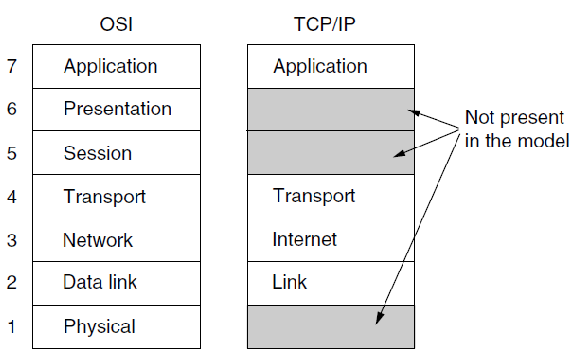
\includegraphics[width=0.309\textwidth]{pic/CN1/The TCPIP Reference Model}
    \caption{The TCP/IP Reference Model}
\end{figure}

\paragraph{The link layer} 包交换
\paragraph{The Internet layer} IP, ICMP 协议
\paragraph{The transport layer} TCP, UDP 协议
\paragraph{The application layer} DNS (map host names onto their network address) 协议

\begin{figure}[!htb]
    \centering
    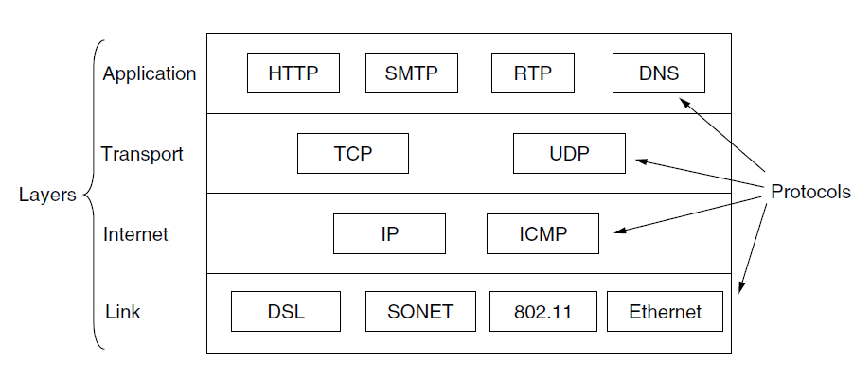
\includegraphics[width=0.309\textwidth]{pic/CN1/study.png}
    \caption{\small The TCP/IP model with some protocols we will study}
\end{figure}

\subsubsection{The OSI vs. TCP/IP}
TCP/IP模型在网络层仅支持一种模式(无连接), 但在传输层同时支持这两种模式. 

\subsection{Standardization}
Two categories: de facto and de jure. (先实践 or 先理论)

\subsection{Metric Units} 
\begin{figure}[!htb]
    \centering
    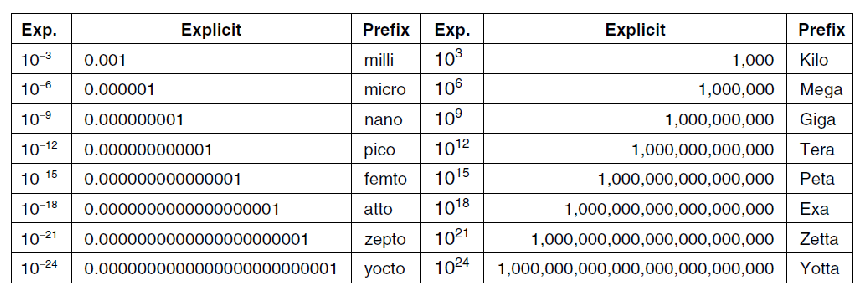
\includegraphics[width=0.42\textwidth]{pic/CN1/Metric prefixes.png}
    \caption{The principal metric prefixes}
\end{figure}

\subsubsection{The Performance of Packet-Switching Networks}
Quantitative Metrics
\begin{itemize}
    \item Delay
    \subitem Processing delay: 检查数据包的标头并确定将数据包去向所需的时间
    \subitem Queuing delay: 计算排队时间
    \subitem Transmission delay: 包长度/速率
    \subitem Propagation delay: 路由间距/传输速度
    \item Loss: buffer 满了就丢包
    \item \textbf{Throughput}(吞吐量): 取决于瓶颈链路(the bottleneck link)的传输速率(最慢的)
\end{itemize}


